\chapter{X-ray and Neutron Scattering}
\label{Chap:diffraction}

\section{Terminology: \texorpdfstring{$2\theta$}{2theta} and Q}

Diffraction is a quantum phenomenon that requires a particle/wave that has a wavelength that is similar in magnitude to the features that one wants to detect. For diffraction from atoms, this means a wavelength similar to the distance between atoms (Ãngstroms) or less. Diffraction measurements are routinely done with x-rays (photons) or neutrons, but not only with these. Increasingly, crystallography is being done with electrons, traditionally with an electron microscope, but some newer instruments are optimized specifically for electron diffraction. Scattering of alpha particles or neutral atoms is sometimes performed – but not for crystallography, e.g. structural information on the arrangement of atoms. Also, though not considered here, muon scattering can be valuable for magnetic studies. I will use the term quantum particles to discuss features that x-rays, neutrons, and electrons all share, but it is worth noting that for diffraction studies, energies needed for neutrons, x-rays and electrons are typically mili-eV, kilo-eV and mega-eV, respectively, to generate wavelengths that are on the order of 1 Å.

One of the most fundamental concepts in scattering is what physicists call momentum transfer: a measure of the deflection of the diffracted quantum particle from that of the impinging beam. This angle is for historical reasons described as $2\theta$ and is usually measured in degrees. 
 Thus, forward scattering, where the particle does not have its scattering direction changed, will have a $2\theta$ value of zero. Complete backscattering, where the particle is scattered back towards the source will have $2\theta=180^\circ$. 
 The $2\theta$ value itself is not useful without knowing the wavelength used. Further, an important class of diffraction measurements is done with energy-dispersive diffraction, where instead of measuring scattering at a fixed wavelength while varying the angle, the measurements are made at a fixed scattering angle as a function of wavelength. Thus, it is best to get away from angular values and use an absolute term that removes the wavelength dependence. Traditionally, crystallographers have used the quantity $\sin\theta/\lambda$ for this but that sees little use, Physicists use a related quantity Q\index{$\rm Q$|textbf}, where $Q =  4 \pi \sin\theta/\lambda$. I am a chemist by training and self-identify as a crystallographer, but I prefer Q over $\sin\theta/\lambda$ due to its more wide-spread acceptance. 


\section{The physics of scattering}

In order to understand diffraction, we need to consider how our probe particle (an x-ray photon, electron, or neutron) interacts with an atom. 
When this quantum particle encounters an atom, it may or may not scatter from that atom. The probability of scattering depends on the type of particle, the type of atom it scatters from, and the energy (wavelength) of that particle. When a photon, electron, or neutron is scattered, there are a total of four different types of scattering that can occur. First of all, there are two modes for scattering with regard to energy exchange: elastic and inelastic. Secondly, since the scattering particle has a phase, it is possible for the phase of the particle to retain that phase, which is known as coherent scattering. Alternately, the phase can be randomized in the process of scattering, which is incoherent scattering. These are quantum-mechanical properties and don't have direct analogs in the world we live in, but the best analogy I can make would be to consider scattering of a tennis ball by a tennis racket. Consider the speed of the tennis ball: Does it leave the racket with the same speed it had before? If the speed changes, the scattering is inelastic. From a physics perspective, in elastic scattering, the quantum particle leaves the atom with no interchange of energy and thus, it has exactly the same energy as it started with, though its direction is usually changed through an exchange of momentum. If the scattering is inelastic or quasi-elastic, the scattered particle transfers energy to (or from) the atom it scatters from. In most cases, the scattered particle loses energy and atoms in the sample receive energy from this process, but for scattering of thermal neutrons, which have energies comparable to atomic vibrational modes, for atoms can transfer energy \textit{to} the scattering particle. In either case, the particle’s energy changes, which results in a wavelength change. 

Absorption is the extreme case of inelastic scattering, where all of the probe particle's energy is lost. Absorption of neutrons leads to neutron activation, where excited nuclear states are created, these may decay immediately or become new elements or isotopes. If the new isotope is radioactive, the half-life can be of any length, from tiny fractions of a second to millennia. With x-rays, photon absorption can be followed by emittance of a lowered energy photon (Compton scattering) or can involve an electronic resonance resulting in fluorescence. When x-ray scattering results in a net transfer of energy to the atom, this energy can cause ejection of an electron (ionization) or can cause localized heating, or both. Either can degrade the material, which is known as beam damage. X-ray and neutron absorption also cause biological damage to living tissue, which is why we must protect ourselves from any \textit{appreciable} exposure to these phenomena. Note that we will be always exposed to some non-negligible levels of radiation. This is in part from natural sources, but also from very beneficial medical procedures. A less welcome contribution is from radioactive fallout due to past use of nuclear weapons and other forms of nuclear pollution.

To provide an analogy for coherent vs. incoherent scattering, consider the timing for the arrival of our tennis ball. If the ball bounces off the racket instantaneously, this is coherent scattering. The timing is unchanged. 
However, for incoherent scattering, consider what happens if the tennis ball spends some time on the racket before leaving.  (Envision a Velcro wrapping on the racket?) At this point, we have lost track of the timing for our tennis ball. This matters because, considering wave-like interactions, the scattering from this particle will no longer be able to interact with other particles. 
From a physics perspective, in coherent scattering, the wavefunction of the incident particle is changed in a systematic way by the interaction with the atom. We describe this wavefunction as having a phase. In coherent scattering, the phase may be unchanged by the interaction with the atom, or it may be inverted. In contrast, with incoherent scattering, the phase of the quantum particle is randomized in the scattering event. 
In fact, the quantum world behaves with very different rules than the macroscopic one we live in, and the phase of a particle is best described as a complex quantity – complex meaning a special type of 2D vector having components in two different directions, where numbers can be written as $z = x + iy$ where $i=\sqrt{-1}$. Here $x$ is called the \textbf{real }\textbf{component} and $y$ the \textbf{imaginary }\textbf{component}. That the phase is a complex quantity, which will become important as we consider scattering at resonance edges for atoms. 

All four combinations of the two types of scattering occur. For diffraction, we only want scattering that is elastic and coherent, but it is worthwhile to understand the other three combinations:  the other scattering modes can provide different types of information, and these are utilized via a plethora of non-diffraction techniques such as XAFS, inelastic neutron scattering, EELS, and even prompt-neutron activation analysis, to name just a few from a long list. These other scattering/absorptive processes may degrade the quality of a diffraction experiment, in some cases significantly. As an example, for each element, there are edges where x-ray absorption increases dramatically. Above these edges, many of the incident x-rays are re-emitted at different wavelengths via fluorescence, which thus increases dramatically the background scattering coming from the sample, which reduces our ability to measure the diffraction signal precisely unless our x-ray detection system is able to filter this out. As another example, \textsuperscript{1}H (hydrogen as opposed to deuterium) scatters neutrons incoherently more than 100 times stronger than most atoms can scatter neutrons coherently. This means if a sample contains just a few atom percent \textsuperscript{1}H, (which corresponds to an even tinier fraction by weight/mass,) one will see the incoherent scattering as background, which again reduces the measurement signal-to-noise. 

\section{Scattering Probabilities}

To compute scattering, we need to tabulate the probability for scattering of our probe by atoms. This probability function is described with several names and formulations.

\subsection{X-ray Form Factors}

For x-rays, the probability for scattering is usually called the form factor\index{form factor|textbf} and is written as \textit{f}($2\theta$) or \textit{f}(Q), with units of length. X-ray photons are predominantly scattered by the electrons in an atom, and since the electrons are smeared out across a large region of the atom, the probability for interaction is greatest when the electron has the greatest average path through the atom -- which means that the greatest scattering probability is for forward scattering, where the momentum (path) of the photon is not changed. The form factor for forward scattering, \textit{f}(0), is proportional to the number of electrons in the atom or ion and by convention\textit{f}(0)=Z where Z is the number of electrons for the species. The larger the angle of scattering, the lower the probability of scattering. The probability of scattering thus is a function of the scattering angle but if tabulated as a function of Q (or equivalently $\sin\theta/\lambda$) is largely independent on the energy of the photon. Form factor values are computed for isolated atoms using high-level quantum theory (typically Hartree-Fock) and are tabulated in the International Tables for Crystallography Volume C, but in GSAS-II form factors are computed for the specified x-ray wavelength from a set of coefficients tabulated by D. T. Cromer and J. T. Waber (1971) in the International Tables Vol. IV. 

These form factors are only an approximation, since bonding considerations in the solid state do affect the distribution of electrons significantly. Thankfully, bonding most greatly affects the valence electrons, which are already quite diffuse, so even though these form factors are from idealized computations, made for isolated atoms in vacuum, rather for the actual environment of an atom in a real material, they do work pretty well. There are more complex treatments available for fitting diffraction data, but they can only be used with extremely accurate data collected over a very wide Q range. At the time that I write this, the capability to treat non-spherical atom scattering is being added to GSAS-II, but is not yet complete. However, it is not clear if powder diffraction studies will ever be made at sufficient precision to detect the differences between spherical and non-spherical scattering contributions.

A more controversial question is how to describe atoms with formal non-zero oxidation states: should one use scattering factors computed for ions or for neutral atoms? I side with the neutral atom choice. To illustrate why, consider a mixed iron oxide where Fe is nominally Fe\textsuperscript{+3}. The picture taught in first-year chemistry is that Fe has transferred three electrons to neighboring O atoms, However, is not an accurate picture of the chemical bonding, as the electrons are shared in molecular orbitals generated between the Fe and O atoms and on average the valence electrons still have a high probability of being found close to the Fe nucleus. This means that the scattering from this solid-state “ion” is not much changed from that of a neutral Fe atom, as would be by the complete removal of three electrons. My understanding is that even in a highly ionic material such as NaCl, in the solid state, the actual electron density distribution is quite far from what would be the case if there were complete transfer of an electron from each sodium to chlorine. 

Another reason that one may safely use neutral atom scattering factors, even for ions, is that this choice has a very limited impact on the computation. We can understand how the choice of a neutral atom versus a charged-atom species affects the scattering calculation using a utility that GSAS-II offers, where scattering factor curves can be viewed, called PlotXNFF\index{software!PlotXNFF} (found in the Calculate menu). If this is opened, a window labeled “Plot Xray, Neutron and Magnetic Form Factors” is displayed. As an example, click on this window and in the associated menu select the element Fe. This will open a plot where the neutron, x-ray, electron and magnetic scattering factors can be visualized, as seen in the screen image below in Fig. \ref{fig:diff1}. For Q=0, the value will be the number of electrons in the atom, so at 0 degrees (where one cannot measure scattering) \textit{f}(0) for Fe\textsuperscript{+3} is 23 electrons while it is 26 for neutral Fe. The differences between the Fe and Fe\textsuperscript{+3} scattering factor curves become increasingly close as Q increases from zero. Note that by $\sin\theta/\lambda=0.1$ (Q=0.6) the curves for the ionic forms of Fe and the neutral element have largely converged and above double that value the curves are largely indistinguishable. Since few materials have more than a few diffraction peaks at these low values of Q and many small-cell materials have none, computed diffraction patterns will show very slight – if any – differences between neutral and ionic treatment of atomic scattering. Thus, there is very little reason in my opinion to use charged atom form factors. Not only are they a better chemical description of the electron distribution, they are simpler. Based on what we have now seen, they will not change the fitting appreciably.

\begin{figure}
    \centering
    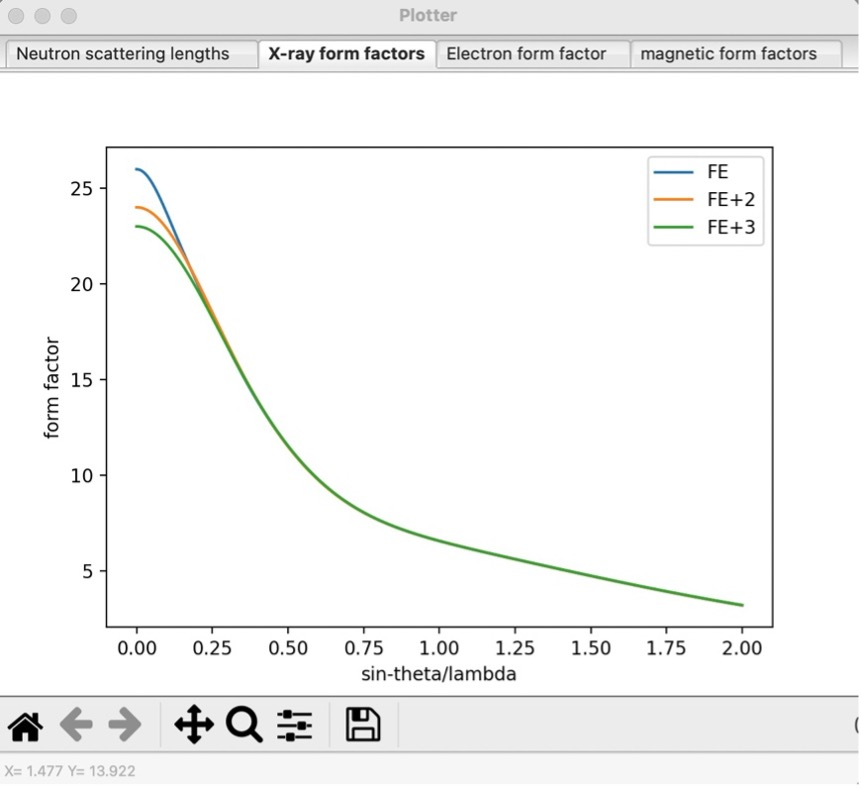
\includegraphics[width=0.6\linewidth]{figures/Diffract1.jpg}
    \caption{Plot of x-ray form factors for Fe, Fe\textsuperscript{2+} and Fe\textsuperscript{3+} from GSAS-II program PlotXNFF}
    \label{fig:diff1}
\end{figure}
Despite my comments, if one persists in using charged-atom scattering factors, a common question will be ``what should I use for a species that is not provided, such as Fe\textsuperscript{+4}?'' Certainly, form factors for Fe\textsuperscript{+3} and Fe\textsuperscript{+4} will be just about the same except at very low Q. Feel free to substitute a similar valence scattering factor curve. Achieving charge balance for scattering factor selection is not important, since again this only affects low-angle scattering and again only in a second-order fashion. 

\subsection{Neutron Scattering Cross Sections}

 In contrast to x-rays, neutrons are usually scattered from the nucleus of the atom, and this scattering can usually be considered as a point-point interaction that does not vary with the angle of scattering. The probability for this type of scattering is thus a constant independent of angle, but does depend on the neutron energy and, in particular, on the interactions at the quantum level between the nucleus of the atom and the neutron, which depends on the isotope of the atom. In fact, the scattering probability may be very different for isotopes of the same element. The scattering probability for neutrons is commonly referenced as a cross-section, $\sigma$,\index{scattering cross-section} with units of area (length\textsuperscript{2}). There is also a quantity related to the square-root of the cross-section, which is called the scattering length, \textit{b},\index{scattering length} and has units of length. Finally, while all atoms scatter x-rays with no phase inversion, most isotopes do scatter neutrons with phase inversion, but a few do not. For those unusual isotope types that do not invert the scattering phase, we indicate this using a negative value for \textit{b}. 

There are separate probabilities for coherent and incoherent neutron scattering, which can vary greatly. As a fairly extreme example, the coherent and incoherent scattering lengths for the \textsuperscript{1}H isotope of hydrogen are -3.7406 fm and 25.274 fm, respectively. Since scattering probabilities go as the square of the scattering lengths, a neutron is $\approx$45 times more likely to be scattered incoherently than coherently by a \textsuperscript{1}H atom. As was discussed previously, this incoherent scattering occurs at all diffraction angles and adds greatly to the background, making it much harder to measure diffraction with significant precision in the presence of a significant atomic percentage of \textsuperscript{1}H. For this reason, samples containing deuterium (\textsuperscript{2}H), for which the coherent and incoherent scattering lengths are 6.671 fm and 4.04 fm, respectively, are greatly preferred for neutron diffraction. 

Noting that almost all elements exist as a mixture of isotopes, the net coherent scattering from any element is dependent on the weighted sums of the scattering lengths, which can work towards canceling each other if the signs of \textit{b} are opposite. While normally \textsuperscript{2}H is only 0.015\% of the natural isotopic makeup of hydrogen, if we enrich the level of \textsuperscript{2}H to 36\% at a site, we have a net coherent scattering of 0.0075 fm [ = (‑3.7406*0.64) + (6.671*0.36)], meaning that there is nearly no coherent scattering from this site. The overall probabilities for scattering from the \textsuperscript{1}H and \textsuperscript{2}H atoms are unchanged by their mixture, but all of their scattering now becomes incoherent. A similar effect occurs with vanadium, which at natural isotopic composition is 0.25\% \textsuperscript{51}V with \textit{b}= 7.6 fm and the remainder \textsuperscript{50}V with \textit{b} = -0.402 fm. Note that (0.25*7.6 + 99.75*-0.402)/100 = ‑0.382 fm, which is a relatively weak diffracting material. Vanadium is a preferred as a container material for neutron diffraction, due to the very small levels of diffraction seen from that metal. 

Note that there are potentially two ways that incoherent scattering can arise. It can be an intrinsic property of the neutron-nucleus interaction, typified by \textsuperscript{1}H, but can also arise from having a mixture of isotopes. GSAS-II provides coherent neutron scattering lengths for elements at natural abundance and for isotopes where the scattering lengths have been reported in the literature, so it is not necessary to look up any of these values.

There is one common exception to the angular-independent scattering of neutrons by atoms, and that occurs in materials with ordered unpaired electrons. Depending on the type of ordering, materials with unpaired electrons may be ferromagnetic, paramagnetic or exhibit related types of magnetic phenomena such as ferrimagnetism. Unpaired electrons have a net spin, as do neutrons, and these unpaired electrons can scatter neutrons from this spin-spin interaction. These unpaired electrons are always valence electrons and thus are more dispersed from the nucleus than the average for all the electrons. This means that scattering of neutrons by unpaired electrons falls with increasing angle similarly to what is seen in x-ray scattering, but the decrease with Q is even faster for magnetic neutron scattering than what is seen in the form factor for x-rays. Different scattering length curves are tabulated for different valence states for atoms that exhibit magnetic effects. These are automatically assigned in GSAS-II when a material with magnetic scattering is defined. 
In GSAS-II to change the valence state for an atom, click on the type entry in the Atoms table. This brings up a periodic table and under each element there are choices for valence state.

\section{Resonant scattering}

As mentioned previously, scattering from an atom involves components in the real and complex planes. This becomes of particular importance when considering scattering at resonant edges, meaning where the energy of an x-ray photon is close to that for an absorption edge for a particular element. When x-rays are scattered near an atom’s absorption edge, the scattering can be described by adding two additional components for scattering in the real and imaginary planes, so the total form factor f\textsubscript{tot}($\lambda$,Q) is written as \textit{f}\textsubscript{tot}($\lambda$,Q) = \textit{f}(Q) + \textit{f}’($\lambda$) + \textit{i}\textit{f}’’($\lambda$). This effect of wavelength on scattering is usually called anomalous dispersion in chemical crystallography and resonant scattering in physics.\index{anomalous dispersion|textbf}\index{resonant scattering|textbf}\label{ref:resonantscattering} I think that resonant scattering seems a much better term to use. The values of \textit{f}’ and \textit{f}’’ are normally quite small, but can reach an electron or two close to absorption edges, which means they are still not large, but do become experimentally significant. 

In a resonant scattering experiment, one collects two datasets, one at a wavelength close to (but still somewhat below) an absorption edge for an element and another at a similar wavelength, but well away from an absorption edge. Since the only significant change between the two patterns will be the scattering from the element at this selected edge. This “tweaking” of the scattering for a particular element can be thought of as akin to the derivative of the diffraction pattern with respect to the element in question, but in GSAS-II one analyzes the data by fitting both datasets against a single model. Note that the values for f’ and f’’ and in particular the exact location of the absorption edge will be dependent on the chemical environment for the selected element, but 100 eV below the edge, the values are pretty much independent of the bonding details. 
Prior to synchrotrons, resonant scattering diffraction experiments were nearly impossible, now they are possible, but are still uncommon as few if any synchrotron diffraction beamlines are designed to change x-ray wavelengths easily. 

 In GSAS-II the values for \textit{f}’ and \textit{f}’’ are computed using the tabulation of D.T. Cromer and D. A. Liberman and are automatically computed for every appropriate element based on the supplied x-ray wavelength. The GSAS-II program Fprime\index{software!Fprime} (in the Calculate menu) shows the values computed with this tabulation as a function of x-ray wavelength. As noted, these values are only approximate near the edge, but where resonant scattering measurements are normally made, circa 100 eV below the resonant scattering edge, the values are largely not highly dependent on the species’ chemical environment and should be reasonable approximations. If greater accuracy is needed, when a resonant scattering experiment is done, one should consider collecting a wavelength-dependent fluorescence or absorption measurement. From this using a Kramers-Kronig inversion one can compute the \textit{f}’ and \textit{f}’’ curves for the specific material being studied as a function of wavelength. This would need to be done outside of GSAS-II. 

 A similar resonant scattering effect can also occur when neutron energies that match absorption edges for particular isotopes, but this is far less common and typically occurs at relatively high neutron energies that are seldom accessible in diffraction experiments, but there are a small number of elements that offer exceptions. GSAS-II uses tables computed by Lynn and Seeger to compute nuclear resonant scattering. The values generated from those tables can be also viewed in program PlotXNFF, as shown in Fig. \ref{fig:diff2}. Nuclear resonant scattering is usually an issue only with the higher energy neutrons available at spallation sources, but that can pose a problem since some TOF instruments sum together data acquired over a wide of range of detector angles. This mixes together diffraction from different wavelengths making treatment of resonance in the form factor impossible. 

 \begin{figure}
    \centering
    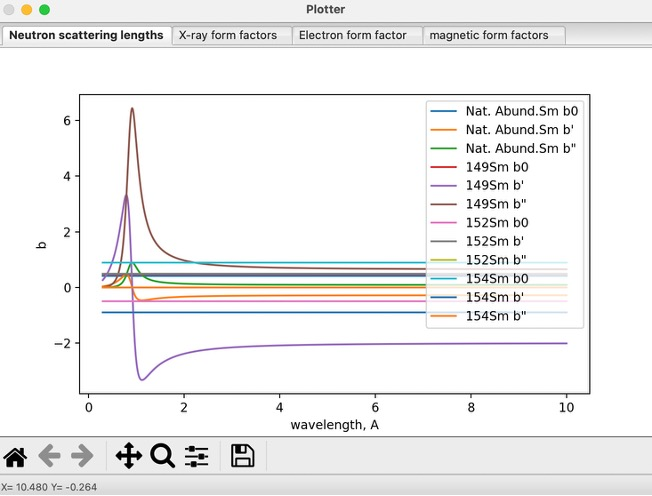
\includegraphics[width=0.6\linewidth]{figures/Diffract2.jpg}
    \caption{Resonant neutron scattering for isotopes of Sm as a function of wavelength as plotted by program PlotXNFF}
    \label{fig:diff2}
\end{figure}

\section{Diffraction from materials}

 Diffraction occurs when a pair of atoms are spaced apart so that their scattering is in phase and thus can add at an appropriate angle. At other angles, the scattering will not have this constructive interference and will on average cancel. A completely random arrangement of atoms would have pairs of atoms at all distances and thus would be expected to have completely uniform diffraction (following the form of \textit{f} with angle) at all scattering angles. However, matter never has a completely random arrangement of atoms. Even gases have some ordering, since atoms can never approach too closely and thus even diffraction from gases will show some level of structure. 
 
Peter Debye\index{Debye, P.} in 1915 first tabulated an equation that computed diffraction intensity as a function of the distances between pairs of atoms in a sample. His equation can be rewritten in a slightly different but more convenient form as: \index{Debye equation|textbf}
$$I\left(Q\right)=Nf^2\sum_{i}^{N}\sum_{j\neq i}^{N}\frac{\sin{Qr_{ij}}}{Qr_{ij}}$$
where r\textsubscript{ij} is the distance between atoms i and j. In this equation, \textit{f} indicates the scattering power for each atom, discussed previously as the form factor or scattering length, and \textit{I(Q)} will be the relative intensity for scattering per unit solid angle. N is the total number of atoms and thus this is a double sum that would include \textit{every} pair of atoms in the sample, which is intractable for any reasonable number of atoms. In practice, since the sinc function [$\operatorname{sinc}(q,r) = \sin(qr)/qr$] falls to very small values as qr becomes large, it is not necessary to consider pairs of atoms at very large distances. This equation (or equations derived from the Debye equation) allow for computation of diffraction scattering from disordered materials, such as glasses, but can be simplified greatly for crystalline materials as will be discussed further below. 

\section{Absorption and Extinction}

As we saw before, neutron or x-ray quanta can interact with the sample in several ways. Alternatively, they may also not be scattered at all and go straight through the sample unperturbed. When quanta are scattered incoherently or inelastically or are captured by the sample, they can no longer contribute to the diffraction signal. Diffraction intensities are computed ignoring this effect, but when samples have high probabilities for neutron or x-ray absorption or non-diffraction scattering, the fraction of lost quanta will depend on the scattering geometry, the wavelength and the diffraction angle. If a significant fraction of the quanta are absorbed or are otherwise scattered by non-diffraction events, a correction factor may be needed to accurately match the idealized diffraction intensities to what is actually observed. This is known as an absorption correction, but it should be noted that non-diffraction scattering as well as actual absorption is corrected for in this factor. To evaluate the effects of absorption, GSAS-II includes a program (also in the Calculate menu) called Absorb\index{software!Absorb} where a chemical formula is supplied along with a sample size and density or packing fraction (since powder samples usually are not fully dense) and the value of $\mu r$ is computed as function of wavelength. Absorption corrections are discussed in more depth in \S\ref{ref:Absorption}.

Another assumption that is made when computing diffraction intensities is that the probe quanta are only scattered once and only a small fraction are scattered. In an effect called multiple scattering, it is possible for a scattered quantum to be scattered again before it leaves the sample. This occurs most significantly for intense reflections in large single crystals and this effect is called primary extinction. This effect is greatest when crystals have very large domains, without defects to disrupt ordering. To compute primary extinction quantitatively, one must use a higher level of scattering theory than will be discussed here, called dynamical diffraction. Note that primary extinction can be quite significant in electron diffraction because with the high electron energies used, only small domains within a sample are probed and are much more likely to have “perfect” ordering on these distance scales. 
 
Another effect can occur, similar to absorption, if significant fraction of the incident quanta are diffracted before many of the particles penetrate into the sample. The result of this is that fewer quanta are available to be scattered than will be expected. This is known as secondary extinction. 

Both primary and secondary extinction are most likely to be observed with large and highly perfect crystals. More commonly, so-called single crystals are actually constructed of relatively small domains due to defects and these domains have small misalignments with each other. Such a crystal is known as ideally mosaic. The small domain sizes disrupt the dynamical scattering needed to cause primary extinction and the small misalignments between domains prevent secondary extinction. Single-crystal experiments will sometimes benefit if a crystal is thermally shocked to induce mosaicity. However, extinction is quite rare in powder diffraction because when crystallite sizes are larger than a few microns, sample grinding should be used. GSAS-II does provide correction terms for extinction that can be used for both single-crystal and powder diffraction and with both x-rays and neutron. While rarely needed, these do work well for materials with very large crystallite sizes. Note that laboratory powder diffraction experiments with such large-grain materials are likely to be inaccurate, due to poor particle counting statistics, but this is less likely to be a problem with high-energy x-rays and neutrons.  

\section{For More Information}

\begin{itemize}
\item \textit{Fundamentals of Crystallography.} Third Edition (2011). C. Giacovazzo, H. L. Monaco, G. Artioli, D. Viterbo, M. Milaneso, G. Ferraris, G. Gilli, P. Gilli, G. Zanotti and M. Catti. Edited by C. Giacovazzo. IUCr Texts on Crystallography No. 15, IUCr/Oxford University Press.
\begin{quote}
This is a weighty, comprehensive, and modern book on crystallography. If you are going to buy anything, this is what I would recommend. 
\end{quote}

\item\textit{Elements of X-Ray Diffraction}, 3rd Edition (2014), B.D. Cullity and S.R. Stock. Pearson. 
\begin{quote}
This is a general x-ray diffraction text that is more oriented to materials studies than most. Commonly used as a teaching textbook. Despite the publication date, it was last revised in 2001, I believe.
\end{quote}

\item \textit{International Tables for Crystallography
Volume C: Mathematical, Physical and Chemical Tables}, (2021) T. R. Welberry ed.\\ 
DOI: 10.1107/97809553602060000117
\begin{quote}
This is a comprehensive and pricey reference on all types of diffraction, with tables and articles on practically everything, but is probably much more than you want. Your library/institution may have arranged on-line access, even if they don't have a print copy. 
\end{quote}
\end{itemize}
